\documentclass[
border={-0pt 0pt -0pt 0pt} % left bottom right top
]{standalone} 

% -----------------------
% CONFIG FONTS
%--------------------------
% Choose your font here
\usepackage{cmbright} 	% Sans-serif font similar to LaTeX default. Math mode looks good.
%\usepackage{kpfonts}	% Palatino-like font. Pretty

\usepackage{bm} % Make sure \boldsymbol works


%--------------------------
% Enabling \mathscr{} for pretty calligraphic fonts. :)

\makeatletter
\DeclareFontEncoding{LS1}{}{}
\DeclareFontEncoding{LS2}{}{\noaccents@}
\DeclareFontSubstitution{LS1}{stix}{m}{n}
\DeclareFontSubstitution{LS2}{stix}{m}{n}
\makeatother

\DeclareMathAlphabet\mathscr{LS1}{stixscr}{m}{n}
\SetMathAlphabet\mathscr{bold}{LS1}{stixscr}{b}{n}
\makeatother

% -----------------------
% CONFIG PACKAGES
% -----------------------
% COLORS
\usepackage[dvipsnames]{xcolor}
\usepackage{amsmath}

% -----------------------
% TIKZ PACKAGES
\usepackage{tikz}
\usetikzlibrary{positioning}
\usetikzlibrary{calc,patterns,angles,quotes}%Tikz angles
\usetikzlibrary{decorations.text}
\usetikzlibrary{shapes.misc}
\usetikzlibrary{fadings}




\usetikzlibrary{external}
\tikzexternalize[prefix=./outputs/] % activate and define figures/ as cache folder
\tikzset{external/force remake} % Always force remake in a standalone

% -----------------------
% TIKZ-FEYNMAN

%Feynman Diagrams -- LuaLaTeX compiler needed
\usepackage[compat=1.1.0]{tikz-feynman}
\tikzfeynmanset{/tikzfeynman/warn luatex=false} % Except not really, you can turn off the warning

% Configuration file -- sets the default colours for TIKZ-FEYNMAN elements
%%%%%%%%%%%%%%%%%%%%%%%%%%%%%%%%%%%
% CONFIG FILE FOR TIKZ-FEYNMAN

% ----------------------
% Tikz-Feynman configurations:

% Shorter momentum arrows, farther from the diagram:
\tikzfeynmanset{/tikzfeynman/momentum/arrow distance=3.0mm}
\tikzfeynmanset{/tikzfeynman/momentum/arrow shorten= .30}

% ----------------------
% Momentum arrows in black by default
\tikzfeynmanset{momentum/arrow style = {Black}}


% ---------------------
% DEFINE GHOSTS TO HAVE ARROWS AND ROUND DOTS

\makeatletter
\tikzset{
	dot diameter/.store in=\dot@diameter,
	dot diameter=3pt,
	dot spacing/.store in=\dot@spacing,
	dot spacing=3pt,
	dots/.style={
		line width=\dot@diameter,
		line cap=round,
		dash pattern=on 0pt off \dot@spacing
	}
}
\makeatother

\tikzfeynmanset{
	ghost/.style={
    	/tikz/draw=none,
		/tikz/decoration={name=none},
		/tikz/postaction={
		/tikz/draw,
		/tikz/dots,		%Using /tikz/dots (defined above) instead of /tikz dotted
		/tikz/very thick,
		/tikzfeynman/with arrow=0.5, % Arrow at midpoint of edge
		},
	}
}



% ---------------------
% DEFINE BLOBS

\tikzfeynmanset{
	blob/.style={
		/tikz/shape	= circle,
		/tikz/draw	= black,			% Edge colour
		/tikz/fill	= gray!40,			% Interior colour
		% ---
		/tikz/inner sep 	= 0.25 cm,	% Separation between label and edge (I presume)
		/tikz/minimum size  = 2.00 cm,	% Minimum size, otherwise scales with label
	}
}


%---------------------
% ADD COLORS (OPIONAL)

\tikzfeynmanset{
	% A possible style:
	%gluon/.append style	= {RoyalBlue},
	%momentum/arrow style 	= {Red!80!Black},
	blob/.append style		= {/tikz/draw = RoyalBlue, /tikz/fill = RoyalBlue!20},
}







% -----------------------
% SOME COMMANDS

\newcommand{\mycomment}[1]{}

\newcommand{\sub}[1]{_{#1}^{}} %Subscripts with proper height
\newcommand{\upp}[1]{_{}^{#1}} %Superscripts with proper height
\newcommand{\ind}[2]{^{#1}_{#2}} %Both


%--------------------------
\begin{document}
	
%% Set this figure's name when externalised 
%\tikzsetnextfilename{partonshowermedium-steps} 
\tikzsetnextfilename{partonshowermedium-full-highlight} 

%
\newlength{\QGPlength}\setlength{\QGPlength}{12.00cm}
\newlength{\QGPheight}\setlength{\QGPheight}{9.00cm}
%
% %%%%%%%%%%%%%%%%%%%%%%%%%%%%%%%%%%%%%%%%%%%%%%%%%%%%%%%%%%
% NOTE TO SELF:
% 	IN TEXSTUDIO, COMMENT MULTIPLE LINES AT ONCE WITH CTRL+T
% %%%%%%%%%%%%%%%%%%%%%%%%%%%%%%%%%%%%%%%%%%%%%%%%%%%%%%%%%%
%
\begin{tikzpicture}
\begin{feynman}
		
% Proper size --- Bounding box
\useasboundingbox (0, 0.5*\QGPheight) rectangle (\QGPlength, -0.5*\QGPheight);

% ------------------------------------------------
% COMMENT THESE LINES TO SEE THE INDIVIDUAL STEPS
% ------------------------------------------------	

% QGP Effect
\path[left color=orange!70,right color=white, overlay] (0, 0.5*\QGPheight) rectangle (\QGPlength, -0.5*\QGPheight);

% Vacuum emissions
% ---------------------
% Blob & Shower origin
\coordinate (Blob) at (1.20cm,0.00cm);
\path (Blob) +(1.00cm,0.00cm) coordinate (Origin);

% ------------------------------------------------
% Blob Drawing
\vertex[blob] (b) at (Blob) {}; 

% ------------------------------------------------
% Coordinates: Vacuum Shower 

\path (Origin) +(2.00cm,0.00cm) coordinate (PairCreation);

% Main Branches	
\path (PairCreation) +(+30:7.00cm) coordinate (EndUpperBranch);
\path (PairCreation) +(-30:7.00cm) coordinate (EndLowerBranch);

\path (EndUpperBranch) +(+20:1.50cm) coordinate (UpperGluon);
\path (EndUpperBranch) +(-40:1.50cm) coordinate (UpperFermion);

\path (EndLowerBranch) +(-35:1.50cm) coordinate (LowerGluon);
\path (EndLowerBranch) +(+20:1.50cm) coordinate (LowerFermion);

% 'First Emission' branch
\path (PairCreation) +(+30:0.75cm) coordinate (Emission1);
%
\path (Emission1) +(+00:2.50cm) coordinate (Gluon1);
%
\path (Gluon1) +(+15:2.00cm) coordinate (Gluon1a);
\path (Gluon1a) +(+10:2.50cm) coordinate (Fermion1a);
\path (Gluon1a) +(-10:2.50cm) coordinate (Fermion1b);
%
\path (Gluon1) +(-20:3.00cm) coordinate (Gluon1b);
\path (Gluon1b) +(+15:1.75cm) coordinate (Gluon1c);			
\path (Gluon1b) +(-15:1.75cm) coordinate (Gluon1d);			

% 'Second Emission' branch
\path (PairCreation) +(-30:5.25cm) coordinate (Emission2);
%
\path (Emission2) +(+20:2.00cm) coordinate (Gluon2);
%
\path (Gluon2) +(+15:1.00cm) coordinate (Fermion2a);	
\path (Gluon2) +(-10:1.00cm) coordinate (Fermion2b);	

% ------------------------------------------------
% Diagram: Vacuum Shower
\diagram*{
	
	% Main branches and pair creation 	
	(Origin) -- [photon] (PairCreation),
	
	(LowerFermion)	-- [fermion] (EndLowerBranch)
	-- [fermion] (PairCreation) 
	-- [fermion] (EndUpperBranch) 
	-- [fermion] (UpperFermion),
	
	(UpperGluon) -- [gluon] (EndUpperBranch),
	(LowerGluon) -- [gluon] (EndLowerBranch),
	
	% 'First Emission' branch
	(Emission1) -- [gluon] (Gluon1) 
	-- [gluon] {(Gluon1a), (Gluon1b)},
	
	(Fermion1b) -- [fermion] (Gluon1a)
	-- [fermion] (Fermion1a),
	
	{(Gluon1c), (Gluon1d)} -- [gluon] (Gluon1b),
	
	% 'Second Emission' branch
	
	(Emission2) -- [gluon] (Gluon2),
	
	(Fermion2a) -- [fermion] (Gluon2) 
	-- [fermion] (Fermion2b),
	
};

	
% Medium induced emissions
% ------------------------------------------------
% Coordinates: Medium-induced emissions

% Induced upper branch	
\path (PairCreation) +(+30:4.50cm) coordinate (InducedEmission1);
%
\path (InducedEmission1) +(-10:2.50cm) coordinate (InducedGluon1);
%
\path (InducedGluon1) +(+15:1.00cm) coordinate (InducedFermion1a);	
\path (InducedGluon1) +(-10:1.00cm) coordinate (InducedFermion1b);	

% Induced lower branch	
\path (PairCreation) +(-30:2.00cm) coordinate (InducedEmission2);
%
\path (InducedEmission2) +(-65:3.50cm) coordinate (InducedGluon2);


% ------------------------------------------------
% Diagram: Medium-induced emissions
\diagram*{
			
	% Induced upper branch	
	(InducedEmission1) -- [gluon] (InducedGluon1),
	
	(InducedFermion1a)	-- [fermion] (InducedGluon1) 
	-- [fermion] (InducedFermion1b),
	
	% Induced lower branch	
	(InducedGluon2) -- [gluon] (InducedEmission2),	

};

% Medium collisions
% ------------------------------------------------
% Coordinates: Medium collisions

% Upper branch collision
\path (PairCreation) +(+30:2.50cm) coordinate (CollEnd1);
%
\path (CollEnd1) +(90:0.90cm) coordinate (CollInit1);
%
\path (CollInit1) +(160:0.75cm) coordinate (CollIncoming1);	
\path (CollInit1) +(030:0.75cm) coordinate (CollOutgoing1);	

% Middle branch collision
\path (Gluon1) +(-20:1.50cm) coordinate (CollEnd2Aux);
\path (CollEnd2Aux) +(0cm,-0.08cm) coordinate (CollEnd2); % Because gluons curl
%
\path (CollEnd2) +(-90:0.90cm) coordinate (CollInit2);
%
\path (CollInit2) +(200:0.75cm) coordinate (CollIncoming2);	
\path (CollInit2) +(-30:0.75cm) coordinate (CollOutgoing2);		

% Lower branch collision
\path (PairCreation) +(-30:0.70cm) coordinate (CollEnd3);
%
\path (CollEnd3) +(-90:0.90cm) coordinate (CollInit3);
%
\path (CollInit3) +(200:0.75cm) coordinate (CollIncoming3);	
\path (CollInit3) +(-30:0.75cm) coordinate (CollOutgoing3);		

% ------------------------------------------------
% Diagram: Medium collisions

\diagram*{
	
	% Upper branch collision
	(CollEnd1) -- [gluon] (CollInit1),
	
	(CollIncoming1)	-- [fermion] (CollInit1) 
					-- [fermion] (CollOutgoing1),
	
	% Middle branch collision
	(CollEnd2) -- [gluon] (CollInit2),
	
	(CollIncoming2)	-- [fermion] (CollInit2) 
					-- [fermion] (CollOutgoing2),
	
	
	% Lower branch collision
	(CollEnd3) -- [gluon] (CollInit3),
	
	(CollIncoming3)	-- [fermion] (CollInit3) 
					-- [fermion] (CollOutgoing3),

};

% Medium Recoils
% ------------------------------------------------
% Coordinates: Medium recoil

\path (CollOutgoing1) +(120:0.70cm) coordinate (RecoilIncoming1);
\path (CollOutgoing1) +(005:1.30cm) coordinate (RecoilOutgoing1);

\path (CollOutgoing2) +(220:0.70cm) coordinate (RecoilIncoming2);
\path (CollOutgoing2) +(005:1.30cm) coordinate (RecoilOutgoing2);



% ------------------------------------------------
% Diagram: Medium recoil

\diagram*{

(RecoilIncoming1)	-- [gluon] (CollOutgoing1)
					-- [fermion] (RecoilOutgoing1),

(RecoilIncoming2)	-- [gluon] (CollOutgoing2)
					-- [fermion] (RecoilOutgoing2),


};

% ------------------------------------------------
% Medium recoils dot
\node[red,dot] (RD1) at (CollOutgoing1);
\node[red,dot] (RD2) at (CollOutgoing2);
	
			
\end{feynman}
\end{tikzpicture}

%% Set this figure's name when externalised 
\tikzsetnextfilename{medium-modified-splitting} 
%
\newlength{\length}\setlength{\length}{12.50cm}
\newlength{\height}\setlength{\height}{14.00cm}

\begin{tikzpicture}
	\begin{feynman}
		
	% ---------------------
	% Proper size --- Bounding box
	\useasboundingbox (0, 0.5*\height) rectangle (\length, -0.5*\height);	

	% ----------------
	% M and MDagger
		
	% ---------------------
% Blob & Shower origin
\coordinate (Blob) at (2.50cm,3.00cm);
\path (Blob) +(1.00cm,0.00cm) coordinate (Origin); % Just outside the blob

% ------------------------------------------------
% Blob Drawing
\vertex[blob, thick] (b) at (Blob) {}; 

% ------------------------------------------------
% Splitting
\path (Origin)		+(+00:2.00cm) coordinate (Emission);
\path (Emission)	+(+25:6.50cm) coordinate (GluonEnd);
\path (Emission)	+(-10:6.50cm) coordinate (QuarkEnd);

\node[black,dot] (v) at (Emission);

% ------------------------------------------------
% ------------------------------------------------
% ------------------------------------------------
% Medium modifications


% ----------------------------
% A loop for pre-emission interactions

\path (Origin) +(0.40cm,-0.85cm) coordinate (A1);
\vertex[crossed dot, thick] (a1) at (A1) {};

\path (A1) +(0.00cm,+0.15cm) coordinate (As1);
\path (A1) +(0.00cm,+0.85cm) coordinate (Ae1);

\foreach \i in {2}
{
	
	\pgfmathtruncatemacro{\prev}{\i - 1}; % Compute previous index #RealProgrammingLanguage
	
	\path (A\prev) +(+00:1.20cm) coordinate (A\i); % Next scattering centre
	
	\vertex[crossed dot, thick] (a) at (A\i) {}; % Draw crossed dot
	
	\path (A\i) +(0.00cm,+0.15cm) coordinate (As\i); % Start of exchanged gluons
	\path (A\i) +(0.00cm,+0.85cm) coordinate (Ae\i); % End of exchanged gluons
	
}

% ----------------------------
% A loop for post-emission interactions

% The first quark-medium scattering
\path (Emission) +(0.70cm,-1.00cm) coordinate (Q1);
\vertex[crossed dot, thick] (q) at (Q1) {};

\path (Q1) +(0.00cm,+0.15cm) coordinate (Qs1); % Start of exchanged gluon
\path (Q1) +(0.00cm,+0.87cm) coordinate (Qe1); % End of exchanged gluon

% The first gluon-medium scattering
\path (Emission) +(0.70cm,+1.50cm) coordinate (G1);
\vertex[crossed dot, thick] (g) at (G1) {};

\path (G1) +(0.00cm,-0.15cm) coordinate (Gs1); % Start of exchanged gluon
\path (G1) +(0.00cm,-1.07cm) coordinate (Ge1); % End of exchanged gluon

% ----------
% A LOOP !!!
\foreach \i in {2,...,5}
{

\pgfmathtruncatemacro{\prev}{\i - 1}; % Compute previous index #RealProgrammingLanguage

% -----------
% QUARK

\path (Q\prev) +(-10:1.20cm) coordinate (Q\i); % Next scattering centre

\vertex[crossed dot, thick] (q) at (Q\i) {}; % Draw crossed dot

\path (Q\i) +(0.00cm,+0.15cm) coordinate (Qs\i); % Start of exchanged gluons
\path (Q\i) +(0.00cm,+0.87cm) coordinate (Qe\i); % End of exchanged gluons

% -----------
% GLUON

\path (G\prev) +(+25:1.20cm) coordinate (G\i); % Next scattering centre

\vertex[crossed dot, thick] (g) at (G\i) {}; % Draw crossed dot

\path (G\i) +(0.00cm,-0.15cm) coordinate (Gs\i); % Start of exchanged gluons
\path (G\i) +(0.00cm,-1.07cm) coordinate (Ge\i); % End of exchanged gluons

}



% ------------------------------------------------
% Diagram:
\diagram*{
	
	% --------
	% Emission	
	(Origin) -- [fermion, thick] (Emission) -- [fermion, thick] (QuarkEnd),
	(GluonEnd) -- [gluon, thick] (Emission),

	% --------
	% Scatterings	
	(As1) -- [gluon, thick] (Ae1),
	(As2) -- [gluon, thick] (Ae2),

	\foreach \i in {1,...,5}
	{ 
	(Qs\i) -- [gluon, thick] (Qe\i),	
	(Gs\i) -- [gluon, thick] (Ge\i),
	}	

};
	

	% ---------------------
% Blob & Shower origin
\coordinate (BlobDagger) at (2.50cm,-3.00cm);
\path (BlobDagger) +(1.00cm,0.00cm) coordinate (Origin); % Just outside the blob

% ------------------------------------------------
% Blob Drawing
\vertex[blob, thick] (b) at (BlobDagger) {}; 

% ------------------------------------------------
% Splitting
\path (Origin)		+(+00:4.50cm) coordinate (EmissionDagger);
\path (EmissionDagger)	+(+25:4.00cm) coordinate (GluonEnd);
\path (EmissionDagger)	+(-10:4.00cm) coordinate (QuarkEnd);

\node[black,dot] (v) at (EmissionDagger);

% ------------------------------------------------
% ------------------------------------------------
% ------------------------------------------------
% Medium modifications


% ----------------------------
% A loop for pre-emission interactions

\path (Origin) +(0.40cm,-0.85cm) coordinate (A1);
\vertex[crossed dot, thick] (a1) at (A1) {};

\path (A1) +(0.00cm,+0.15cm) coordinate (As1);
\path (A1) +(0.00cm,+0.85cm) coordinate (Ae1);

\foreach \i in {2,...,4}
{
	
	\pgfmathtruncatemacro{\prev}{\i - 1}; % Compute previous index #RealProgrammingLanguage
	
	\path (A\prev) +(+00:1.20cm) coordinate (A\i); % Next scattering centre
	
	\vertex[crossed dot, thick] (a) at (A\i) {}; % Draw crossed dot
	
	\path (A\i) +(0.00cm,+0.15cm) coordinate (As\i); % Start of exchanged gluons
	\path (A\i) +(0.00cm,+0.85cm) coordinate (Ae\i); % End of exchanged gluons
	
}

% ----------------------------
% A loop for post-emission interactions

% The first quark-medium scattering
\path (EmissionDagger) +(0.70cm,-1.00cm) coordinate (Q1);
\vertex[crossed dot, thick] (q) at (Q1) {};

\path (Q1) +(0.00cm,+0.15cm) coordinate (Qs1); % Start of exchanged gluon
\path (Q1) +(0.00cm,+0.87cm) coordinate (Qe1); % End of exchanged gluon

% The first gluon-medium scattering
\path (EmissionDagger) +(0.70cm,+1.50cm) coordinate (G1);
\vertex[crossed dot, thick] (g) at (G1) {};

\path (G1) +(0.00cm,-0.15cm) coordinate (Gs1); % Start of exchanged gluon
\path (G1) +(0.00cm,-1.10cm) coordinate (Ge1); % End of exchanged gluon

% ----------
% A LOOP !!!
\foreach \i in {2,...,3}
{
	
	\pgfmathtruncatemacro{\prev}{\i - 1}; % Compute previous index #RealProgrammingLanguage
	
	% -----------
	% QUARK
	
	\path (Q\prev) +(-10:1.20cm) coordinate (Q\i); % Next scattering centre
	
	\vertex[crossed dot, thick] (q) at (Q\i) {}; % Draw crossed dot
	
	\path (Q\i) +(0.00cm,+0.15cm) coordinate (Qs\i); % Start of exchanged gluons
	\path (Q\i) +(0.00cm,+0.87cm) coordinate (Qe\i); % End of exchanged gluons
	
	% -----------
	% GLUON
	
	\path (G\prev) +(+25:1.20cm) coordinate (G\i); % Next scattering centre
	
	\vertex[crossed dot, thick] (g) at (G\i) {}; % Draw crossed dot
	
	\path (G\i) +(0.00cm,-0.15cm) coordinate (Gs\i); % Start of exchanged gluons
	\path (G\i) +(0.00cm,-1.10cm) coordinate (Ge\i); % End of exchanged gluons
	
}



% ------------------------------------------------
% Diagram:
\diagram*{
	
	% --------
	% Emission	
	(Origin) -- [fermion, thick] (EmissionDagger) -- [fermion, thick] (QuarkEnd),
	(GluonEnd) -- [gluon, thick] (EmissionDagger),
	
	% --------
	% Scatterings	
	
	(As1) -- [gluon, thick] (Ae1),
	(As2) -- [gluon, thick] (Ae2),
	(As3) -- [gluon, thick] (Ae3),
	(As4) -- [gluon, thick] (Ae4),
	
	\foreach \i in {1,...,3}
	{ 
		(Qs\i) -- [gluon, thick] (Qe\i),	
		(Gs\i) -- [gluon, thick] (Ge\i),
	}	
	
};


	% ----------------
	% LABELS M
	\path (Blob)	+(-2.25cm,+0.00cm) coordinate (LabelM);
	\vertex at (LabelM) {\qquad \scalebox{1.5}{$\mathcal{M}\hphantom{\upp{\dagger}}:$}};

	\path (BlobDagger)	+(-2.25cm,+0.00cm) coordinate (LabelMDagger);
	\vertex at (LabelMDagger) {\qquad \scalebox{1.5}{$\mathcal{M}\upp{\dagger}:$}};

	
	% ----------------
	% LINES
	\path (Emission)		+(0.00cm,+3.00cm) coordinate (StartLineUp);
	\path (Emission)		+(0.00cm,-9.00cm) coordinate (StartLineDown);

	\path (EmissionDagger)	+(0.00cm,+9.00cm) coordinate (EndLineUp);
	\path (EmissionDagger)	+(0.00cm,-3.00cm) coordinate (EndLineDown);
		
	\draw[dashed, thick] (StartLineDown) -- (StartLineUp);
	\draw[dashed, thick] (EndLineDown) -- (EndLineUp);

	% ----------------
	% LABELS
	
	\path (StartLineUp)	+(-0.35cm,+0.30cm) coordinate (LabelT);
	\path (EndLineUp) 	+(-0.35cm,+0.30cm) coordinate (LabelTDagger);
	
	\vertex at (LabelT) {\qquad \scalebox{1.5}{$t$}};
	\vertex at (LabelTDagger) {\qquad \scalebox{1.5}{$t'$}};
		
	\end{feynman}
\end{tikzpicture}

%% Set this figure's name when externalised 
\tikzsetnextfilename{partonshowers-quarkgluonsplitting} 
%
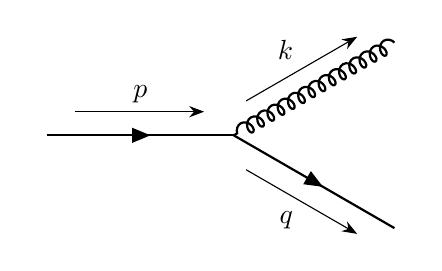
\begin{tikzpicture}
	
	
	% NOTE: MUST *NOT* INCLUDE A {} LABEL FOR THIS ONE
	%		IF A LABEL IS PROVIDED, THERE WILL BE A WHITE CIRCLE OVER THE VERTEX 
	%		USE \node FOR LABELS, \coordinate FOR NO LABEL
	\coordinate (C) at (0,0); 
	
	% Having specified the origin, 
	% the three endpoints are specified in polar coordinates: (angle:radius)
	
	\node (V1) at (180:2.50cm) {};
	\node (V2) at (+30:2.50cm) {};
	\node (V3) at (-30:2.50cm) {};
	
	%%%%%%%%%%%%%%%%%%%%%%%%%%%%%%%%%%%%%%%%%%%%%%%%%%%%%%%%%%%%%%		
	\begin{feynman}
		
		%Diagram
		\diagram*{
			
			(V1) -- [thick, fermion, momentum = \(p\)] (C)
				 -- [thick, fermion, momentum' = \(q\)] (V3),
			
			(V2) -- [thick, gluon, rmomentum' = \(k\)] (C),
			
		};
		
	\end{feynman}
\end{tikzpicture}

%% Set this figure's name when externalised 
\tikzsetnextfilename{partonshowers-quarkgluonsplitting-simple} 
%
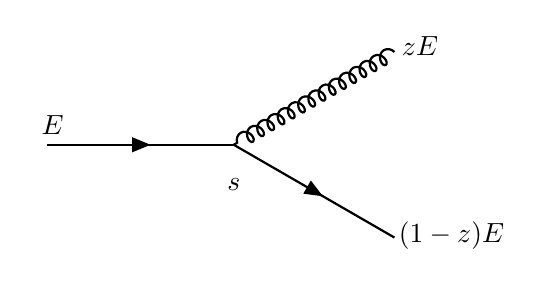
\begin{tikzpicture}
	
	
	% NOTE: MUST *NOT* INCLUDE A {} LABEL FOR THIS ONE
	%		IF A LABEL IS PROVIDED, THERE WILL BE A WHITE CIRCLE OVER THE VERTEX 
	%		USE \node FOR LABELS, \coordinate FOR NO LABEL
	\coordinate (C) at (0,0); 
	
	% Having specified the origin, 
	% the three endpoints are specified in polar coordinates: (angle:radius)
	
	\node (V1) at (180:2.50cm) {};
	\node (V2) at (+30:2.50cm) {};
	\node (V3) at (-30:2.50cm) {};
	
	\node (CLabel) at ($(C)+(0cm,-0.50cm)$) {$s$};
	\node (V1Label) at ($(V1)+(+0.20cm,+0.25cm)$) {$E$};
	\node (V2Label) at ($(V2)+(+0.20cm,0.00cm)$) {$zE$};
	\node (V3Label) at ($(V3)+(+0.60cm,+0.10cm)$) {$(1-z)E$};
	
	
	%%%%%%%%%%%%%%%%%%%%%%%%%%%%%%%%%%%%%%%%%%%%%%%%%%%%%%%%%%%%%%		
	\begin{feynman}
		
		%Diagram
		\diagram*{
			
			(V1)	-- [thick, fermion] (C)
					-- [thick, fermion] (V3),
			
			(V2) -- [thick, gluon] (C),
			
		};
		
	\end{feynman}
\end{tikzpicture}
	
%% Set this figure's name when externalised 
\tikzsetnextfilename{partonshowers-quarkgluonsplitting-labelled} 
%
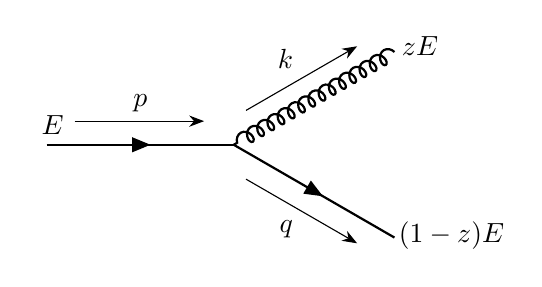
\begin{tikzpicture}
	
	
	% NOTE: MUST *NOT* INCLUDE A {} LABEL FOR THIS ONE
	%		IF A LABEL IS PROVIDED, THERE WILL BE A WHITE CIRCLE OVER THE VERTEX 
	%		USE \node FOR LABELS, \coordinate FOR NO LABEL
	\coordinate (C) at (0,0); 
	
	% Having specified the origin, 
	% the three endpoints are specified in polar coordinates: (angle:radius)
	
	\node (V1) at (180:2.50cm) {};
	\node (V2) at (+30:2.50cm) {};
	\node (V3) at (-30:2.50cm) {};
	
%	\node (CLabel) at ($(C)+(0cm,-0.50cm)$) {$s$};
	\node (V1Label) at ($(V1)+(+0.20cm,+0.25cm)$) {$E$};
	\node (V2Label) at ($(V2)+(+0.20cm,0.00cm)$) {$zE$};
	\node (V3Label) at ($(V3)+(+0.60cm,+0.10cm)$) {$(1-z)E$};
	
	
	%%%%%%%%%%%%%%%%%%%%%%%%%%%%%%%%%%%%%%%%%%%%%%%%%%%%%%%%%%%%%%		
	\begin{feynman}
		
		%Diagram
		\diagram*{
			
			(V1)	-- [thick, fermion, momentum=$p$] (C)
					-- [thick, fermion, momentum'=$q$] (V3),
			
			(V2) -- [thick, gluon, rmomentum'=$k$] (C),
			
		};
		
	\end{feynman}
\end{tikzpicture}	
	
%% Set this figure's name when externalised 
\tikzsetnextfilename{qcdrules-vertexquarkgluon-zoomed} 
%
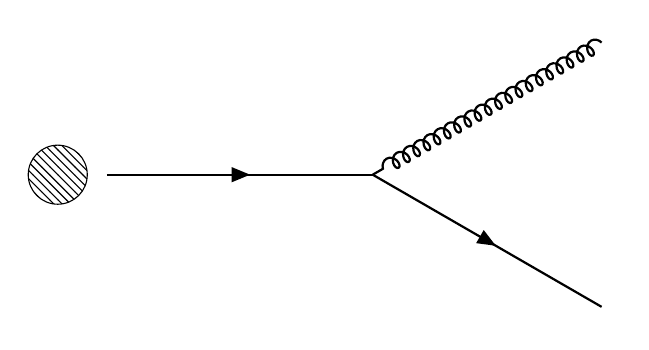
\begin{tikzpicture}
	
	
	% NOTE: MUST *NOT* INCLUDE A {} LABEL FOR THIS ONE
	%		IF A LABEL IS PROVIDED, THERE WILL BE A WHITE CIRCLE OVER THE VERTEX 
	%		USE \node FOR LABELS, \coordinate FOR NO LABEL
	\coordinate (C) at (0,0); 
	\coordinate (Blob) at (-4.00cm,0.00cm);
	
	% Having specified the origin, 
	% the three endpoints are specified in polar coordinates: (angle:radius)
	
	\node (V1) at (180:3.50cm) {};
	\node (V2) at (+30:3.50cm) {};
	\node (V3) at (-30:3.50cm) {};
	
	%%%%%%%%%%%%%%%%%%%%%%%%%%%%%%%%%%%%%%%%%%%%%%%%%%%%%%%%%%%%%%		
	\begin{feynman}
		
		%Diagram
		\diagram*{
			
			(V1) -- [thick, fermion] (C) -- [thick, fermion] (V3),

			(V2) -- [thick, gluon] (C)			
			
		};
		
		\vertex[blob] (b) at (Blob) {\scalebox{1.00}{}}; 
		
	\end{feynman}
\end{tikzpicture}

%% Set this figure's name when externalised 
\tikzsetnextfilename{quark-branch} 
%
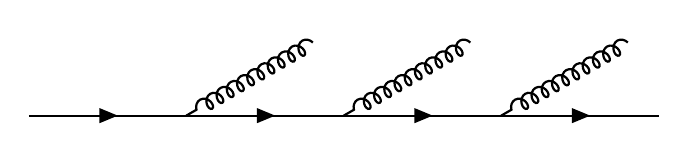
\begin{tikzpicture}
	
	
	% NOTE: MUST *NOT* INCLUDE A {} LABEL FOR THIS ONE
	%		IF A LABEL IS PROVIDED, THERE WILL BE A WHITE CIRCLE OVER THE VERTEX 
	%		USE \node FOR LABELS, \coordinate FOR NO LABEL
	\coordinate (C) at (0,0); 
	
	% Having specified the origin, 
	% the three endpoints are specified in polar coordinates: (angle:radius)
	
	\coordinate (V1) at (0.00cm,0) {};
	\coordinate (V2) at (2.00cm,0) {};
	\coordinate (V3) at (4.00cm,0) {};
	\coordinate (V4) at (6.00cm,0) {};
	\coordinate (V5) at (8.00cm,0) {};
	
	% Specify the gluon nodes as polar coordinates from offset
	
	\node (G2) at ($(V2) + (30:2.00cm)$) {};
	\node (G3) at ($(V3) + (30:2.00cm)$) {};
	\node (G4) at ($(V4) + (30:2.00cm)$) {};
	
	%%%%%%%%%%%%%%%%%%%%%%%%%%%%%%%%%%%%%%%%%%%%%%%%%%%%%%%%%%%%%%		
	\begin{feynman}
		
		%Diagram
		\diagram*{
			
			(V1)	-- [thick, fermion] (V2)
					-- [thick, fermion] (V3) 
					-- [thick, fermion] (V4) 
					-- [thick, fermion] (V5),
						
			(G2) -- [thick, gluon] (V2),		
			(G3) -- [thick, gluon] (V3),			
			(G4) -- [thick, gluon] (V4)			
			
		};
	
	\end{feynman}
\end{tikzpicture}

%% Set this figure's name when externalised 
\tikzsetnextfilename{vertexquarkgluon-wide} 
%
\begin{tikzpicture}
	
	
	% NOTE: MUST *NOT* INCLUDE A {} LABEL FOR THIS ONE
	%		IF A LABEL IS PROVIDED, THERE WILL BE A WHITE CIRCLE OVER THE VERTEX 
	%		USE \node FOR LABELS, \coordinate FOR NO LABEL
	\coordinate (C) at (0,0); 
	
	% Having specified the origin, 
	% the three endpoints are specified in polar coordinates: (angle:radius)
	
	\node (V1) at (180:3.50cm) {};
	\node (V2) at (+40:3.50cm) {};
	\node (V3) at (-40:3.50cm) {};
	
	%%%%%%%%%%%%%%%%%%%%%%%%%%%%%%%%%%%%%%%%%%%%%%%%%%%%%%%%%%%%%%		
	\begin{feynman}
		
		%Diagram
		\diagram*{
			
			(V1) -- [thick, fermion] (C) -- [thick, fermion] (V3),
			
			(V2) -- [thick, gluon] (C)			
			
		};
		
	\end{feynman}
\end{tikzpicture}

%% Set this figure's name when externalised 
\tikzsetnextfilename{vertexquarkgluon-narrow} 
%
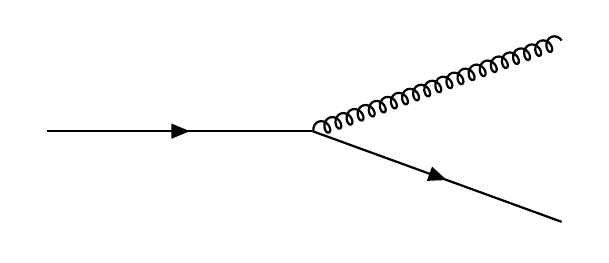
\begin{tikzpicture}
	
	
	% NOTE: MUST *NOT* INCLUDE A {} LABEL FOR THIS ONE
	%		IF A LABEL IS PROVIDED, THERE WILL BE A WHITE CIRCLE OVER THE VERTEX 
	%		USE \node FOR LABELS, \coordinate FOR NO LABEL
	\coordinate (C) at (0,0); 
	
	% Having specified the origin, 
	% the three endpoints are specified in polar coordinates: (angle:radius)
	
	\node (V1) at (180:3.50cm) {};
	\node (V2) at (+20:3.50cm) {};
	\node (V3) at (-20:3.50cm) {};
	
	%%%%%%%%%%%%%%%%%%%%%%%%%%%%%%%%%%%%%%%%%%%%%%%%%%%%%%%%%%%%%%		
	\begin{feynman}
		
		%Diagram
		\diagram*{
			
			(V1) -- [thick, fermion] (C) -- [thick, fermion] (V3),
			
			(V2) -- [thick, gluon] (C)			
			
		};
		
	\end{feynman}
\end{tikzpicture}

% qhat explainer (turned out nice)
%% Set this figure's name when externalised 
\tikzsetnextfilename{partonshowers-singleparton-multiplescatterings} 

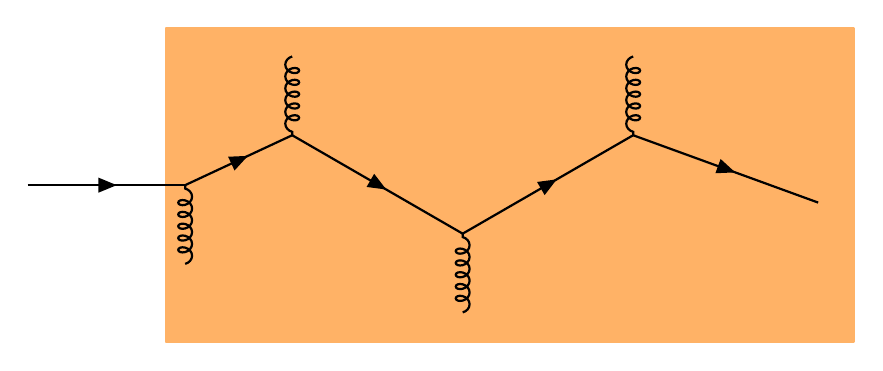
\begin{tikzpicture}

\newlength{\QGPlength}\setlength{\QGPlength}{10.50cm}
\newlength{\QGPheight}\setlength{\QGPheight}{4.00cm}
%
% %%%%%%%%%%%%%%%%%%%%%%%%%%%%%%%%%%%%%%%%%%%%%%%%%%%%%%%%%%
% NOTE TO SELF:
% 	IN TEXSTUDIO, COMMENT MULTIPLE LINES AT ONCE WITH CTRL+T
% %%%%%%%%%%%%%%%%%%%%%%%%%%%%%%%%%%%%%%%%%%%%%%%%%%%%%%%%%%
%
	
	% Proper size --- Bounding box
	\useasboundingbox (0.00cm, 2.00cm) rectangle (10.50cm, -2.00cm);
	
	% ------------------------------------------------
	% COMMENT THESE LINES TO SEE THE INDIVIDUAL STEPS
	% ------------------------------------------------	
	
	% QGP Effect
	\path[left color=orange!60,right color=orange!60] (1.75cm, 2.00cm) rectangle (10.50cm, -2.00cm);
	
	
	% NOTE: MUST *NOT* INCLUDE A {} LABEL FOR THIS ONE
	%		IF A LABEL IS PROVIDED, THERE WILL BE A WHITE CIRCLE OVER THE VERTEX 
	%		USE \node FOR LABELS, \coordinate FOR NO LABEL
	\coordinate (C) at (0,0); 
	
	% Having specified the origin, 
	% the three endpoints are specified in polar coordinates: (angle:radius)
	
	\coordinate (S0) at (2.00cm,0.00cm) {};	
	\coordinate (S1) at ($(S0)+(+25:1.50cm)$) {};
	\coordinate (S2) at ($(S1)+(-30:2.50cm)$) {};
	\coordinate (S3) at ($(S2)+(+30:2.50cm)$) {};
	\coordinate (S4) at ($(S3)+(-20:2.50cm)$) {};

	\coordinate (G0) at ($(S0)+(-90:1.00cm)$) {};
	\coordinate (G1) at ($(S1)+(+90:1.00cm)$) {};
	\coordinate (G2) at ($(S2)+(-90:1.00cm)$) {};
	\coordinate (G3) at ($(S3)+(+90:1.00cm)$) {};

	
	%%%%%%%%%%%%%%%%%%%%%%%%%%%%%%%%%%%%%%%%%%%%%%%%%%%%%%%%%%%%%%		
	\begin{feynman}
		
		%Diagram
		\diagram*{
			
			(C) -- [thick, fermion] (S0)
				-- [thick, fermion] (S1)
				-- [thick, fermion] (S2)
				-- [thick, fermion] (S3)
				-- [thick, fermion] (S4),

			(G0) -- [thick, gluon] (S0),				
			(G1) -- [thick, gluon] (S1),
			(G2) -- [thick, gluon] (S2),
			(G3) -- [thick, gluon] (S3),

			
		};
		
	\end{feynman}
\end{tikzpicture}
	
%% Set this figure's name when externalised 
\tikzsetnextfilename{qcd-antenna-upper-simple} 

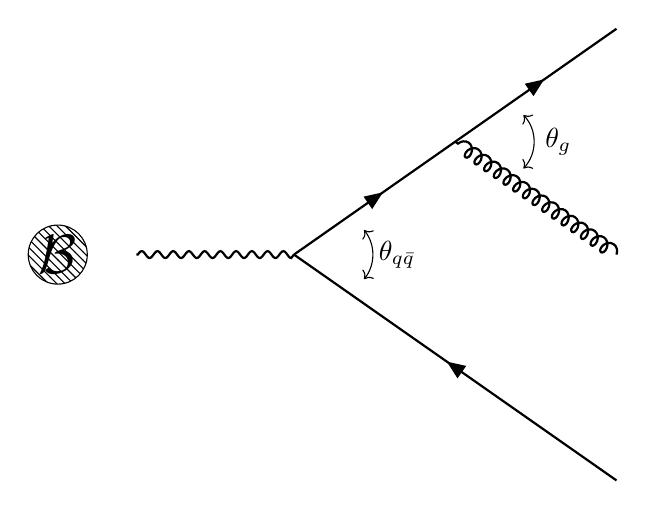
\begin{tikzpicture}
	\begin{feynman}
		
		% ---------------------
		% Blob & Shower origin
		\coordinate (Blob) at (1.20cm,0.00cm);
		\path (Blob) +(1.00cm,0.00cm) coordinate (Origin);
		
		\path (Origin) +(2.00cm,0.00cm) coordinate (PairCreation);
		
		\path (PairCreation) +(+35:2.50cm) coordinate (Emission);
		\path (Emission) 	 +(+35:2.50cm) coordinate (Quark);
		
		\path (PairCreation) +(-35:5.00cm) coordinate (AntiQuark);
		
		\path (Emission) +(-35:2.50cm) coordinate (Gluon);
		
		
		
		% ---------------------	
		\diagram*{
			
			(Origin) -- [thick, photon] (PairCreation),
			
			(AntiQuark) -- [thick, fermion] (PairCreation)
			-- [thick, fermion] 			(Emission)
			-- [thick, fermion] 			(Quark),
			
			(Gluon) -- [thick, gluon] (Emission),
			
		};
		
		% ------------------------------------------------
		% Blob Drawing
		\vertex[blob] (b) at (Blob) {\scalebox{2.00}{$\mathcal{B}$}}; 
		
		% ------------------------------------------------
		% Angles
		\path (PairCreation) +(0:0.50cm) coordinate (PairCreationAngle);
		\pic [draw, <->, "$\,\,\theta_{q\bar{q}}$", angle eccentricity=1.5] {angle = AntiQuark--PairCreationAngle--Quark};    
		
		\path (Emission) +(0:0.50cm) coordinate (EmissionAngle);
		\pic [draw, <->, "$\,\,\theta_{g}$", angle eccentricity=1.5] {angle = Gluon--EmissionAngle--Quark};    
		
		
		
\end{feynman}\end{tikzpicture}	

%% Set this figure's name when externalised 
\tikzsetnextfilename{qcd-antenna-lower-simple} 

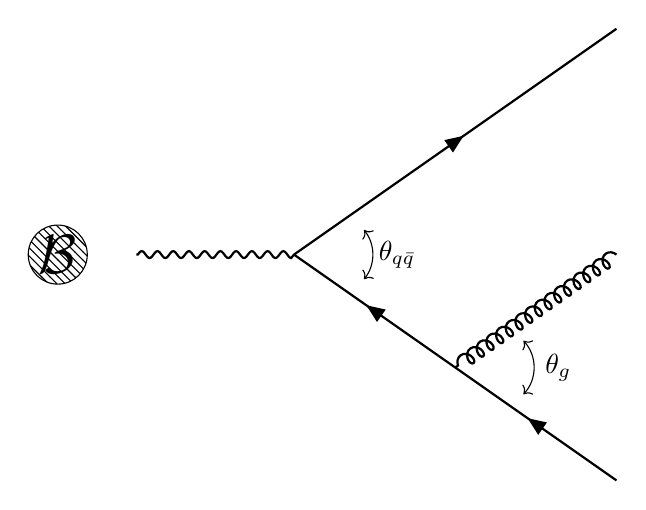
\begin{tikzpicture}
	\begin{feynman}
		
		% ---------------------
		% Blob & Shower origin
		\coordinate (Blob) at (1.20cm,0.00cm);
		\path (Blob) +(1.00cm,0.00cm) coordinate (Origin);
		
		\path (Origin) +(2.00cm,0.00cm) coordinate (PairCreation);
		
		\path (PairCreation) +(+35:5.00cm) coordinate (Quark);
		\path (PairCreation) +(-35:5.00cm) coordinate (AntiQuark);
		
		\path (PairCreation) +(-35:2.50cm) coordinate (Emission);		
		
		\path (Emission) +(+35:2.50cm) coordinate (Gluon);
		
		
		
		% ---------------------	
		\diagram*{
			
			(Origin) -- [thick, photon] (PairCreation),
			
			(AntiQuark) -- [thick, fermion] (Emission)
						-- [thick, fermion] (PairCreation)
						-- [thick, fermion] (Quark),
		
						
			(Gluon) -- [thick, gluon] (Emission),
			
		};
		
		% ------------------------------------------------
		% Blob Drawing
		\vertex[blob] (b) at (Blob) {\scalebox{2.00}{$\mathcal{B}$}}; 
		
		% ------------------------------------------------
		% Angles
		\path (PairCreation) +(0:0.50cm) coordinate (PairCreationAngle);
		\pic [draw, <->, "$\,\,\theta_{q\bar{q}}$", angle eccentricity=1.5] {angle = AntiQuark--PairCreationAngle--Quark};    
		
		\path (Emission) +(0:+0.50cm) coordinate (EmissionAngle);
		\pic [draw, <->, "$\,\,\theta_{g}$", angle eccentricity=1.5] {angle = AntiQuark--EmissionAngle--Gluon};    
		
		
		
\end{feynman}\end{tikzpicture}	

%% Set this figure's name when externalised 
\tikzsetnextfilename{qcd-antenna-sketch} 


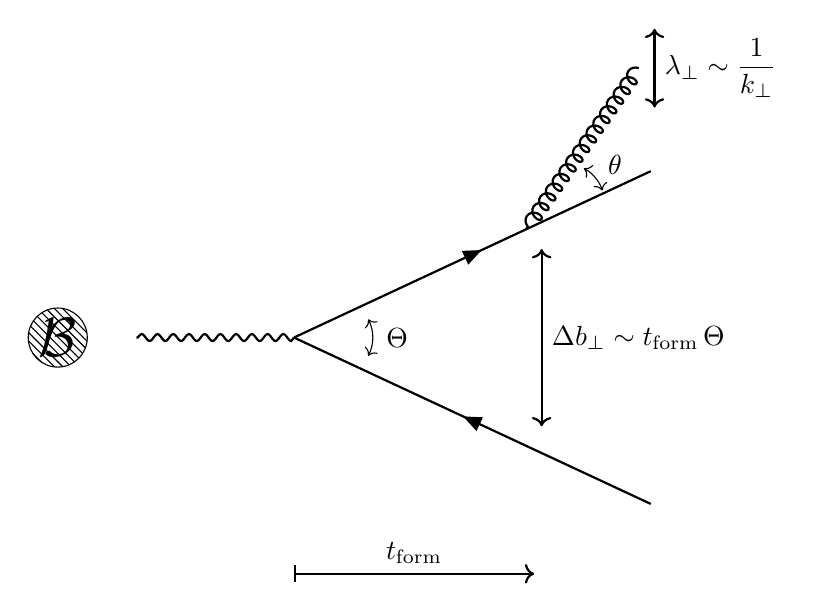
\begin{tikzpicture}
	\begin{feynman}
		
		% ---------------------
		% Blob & Shower origin
		\coordinate (Blob) at (1.20cm,0.00cm);
		\path (Blob) +(1.00cm,0.00cm) coordinate (Origin);
		
		\path (Origin) +(2.00cm,0.00cm) coordinate (PairCreation);
		
		\path (PairCreation) +(+25:5.00cm) coordinate (Quark);
		\path (PairCreation) +(-25:5.00cm) coordinate (AntiQuark);
		
		\path (PairCreation) +(+25:3.25cm) coordinate (Emission);		
		
		\path (Emission) +(+55:2.50cm) coordinate (Gluon);
		
		
		
		% ---------------------	
		\diagram*{
			
			(Origin) -- [thick, photon] (PairCreation),
			
			(AntiQuark) -- [thick, fermion] (PairCreation)
						-- [thick, fermion] (Quark),
						
			
			(Gluon) -- [thick, gluon] (Emission),
			
		};
		
		% ------------------------------------------------
		% Blob Drawing
		\vertex[blob] (b) at (Blob) {\scalebox{2.00}{$\mathcal{B}$}}; 
		
		% ------------------------------------------------
		% Angles
		\path (PairCreation) +(0:0.50cm) coordinate (PairCreationAngle);
		\pic [draw, <->, "$\,\,\Theta$", angle eccentricity=1.5] {angle = AntiQuark--PairCreationAngle--Quark};    
		
		\path (Emission) +(+1.20cm:+0.60cm) coordinate (EmissionAngle);
		\path (Quark) 	 +(-1.20cm:+0.05cm) coordinate (QuarkDraw);
		\pic [draw, <->, "$\,\,\theta$", angle eccentricity=1.5] {angle = QuarkDraw--EmissionAngle--Gluon};    
		
		\coordinate (PairCreationTimeScale) at (4.20cm, -3.00cm);		
		\coordinate (GluonTimeScale) at (7.25cm, -3.00cm);
		\draw [thick, |->] (PairCreationTimeScale)--(GluonTimeScale) node[midway, above] {$t_{\rm form}$};
		
		\path (Gluon) +(0.20cm, +0.50cm) coordinate (GluonUpper);
		\path (Gluon) +(0.20cm, -0.50cm) coordinate (GluonLower);
		\draw[thick, <->] (GluonLower)--(GluonUpper) node[midway, right] {$\lambda_{\perp} \sim \dfrac{1}{k_\perp}$};

		\path (Emission) +(0.20cm, -0.25cm) coordinate (EmissionUpper);
		\path (EmissionUpper) +(0.00cm, -2.25cm) coordinate (EmissionLower);
		\draw[thick, <->] (EmissionUpper)--(EmissionLower) node[midway, right] {$\Delta b_{\perp} \sim t_{\rm form} \, \Theta$};

		
\end{feynman}\end{tikzpicture}	

%% Set this figure's name when externalised 
\tikzsetnextfilename{double-emission-M1} 


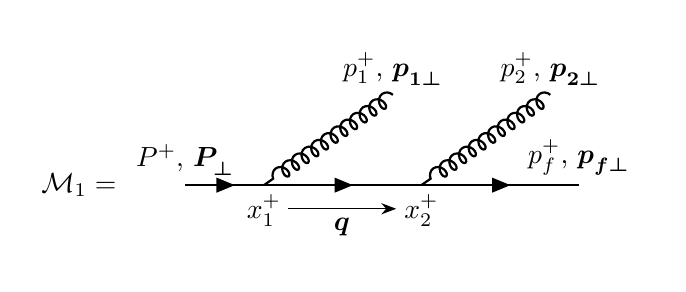
\begin{tikzpicture}\begin{feynman}
		
		% ---------------------
		% Proper size --- Bounding box
		\useasboundingbox (-2.0cm, -1.0cm) rectangle (6.0cm, 2.0cm);	
		
		% ---------------------
		% Blob & Shower origin
		
		\coordinate (Start) at (0.00cm,0.00cm);
		
		\path (Start) +(1.00cm,0.00cm) coordinate (Split1);
		\path (Split1) +(2.00cm,0.00cm) coordinate (Split2);
		\path (Split2) +(2.00cm,0.00cm) coordinate (Quarkf);
		
		\path (Split1) +(35:2.00cm) coordinate (Gluon1);
		\path (Split2) +(35:2.00cm) coordinate (Gluon2);
	
		\vertex[left=0.75cm of Start] (M1) {$\mathcal{M}_1 = $};
		
		\vertex[above=0cm of Start] (Qi) {$ P^{+}_{}\text{, } \boldsymbol{ P_{\perp}^{}} $};
		\vertex[above=0cm of Gluon1] (G1) {$ p^{+}_{1}\text{, } \boldsymbol{ p_{1\perp}^{}} $};
		\vertex[above=0cm of Gluon2] (G2) {$ p^{+}_{2}\text{, } \boldsymbol{ p_{2\perp}^{}} $};
		\vertex[above=0cm of Quarkf] (Qf) {$ p^{+}_{f}\text{, } \boldsymbol{ p_{f\perp}^{}} $};

		\vertex[below=0.0cm of Split1] (S1) {$x^+_1$};
		\vertex[below=0.0cm of Split2] (S2) {$x^+_2$};
		% ---------------------	
		\diagram*{
			
			(Start) -- [thick, fermion] (Split1)
					-- [thick, fermion, momentum'=$ \boldsymbol{ q_{}^{}} $] (Split2)
					-- [thick, fermion] (Quarkf),
			
			(Gluon1) -- [thick, gluon] (Split1),
			(Gluon2) -- [thick, gluon] (Split2),
			
		};
		
		
		
\end{feynman}\end{tikzpicture}

%% Set this figure's name when externalised 
\tikzsetnextfilename{double-emission-M2} 



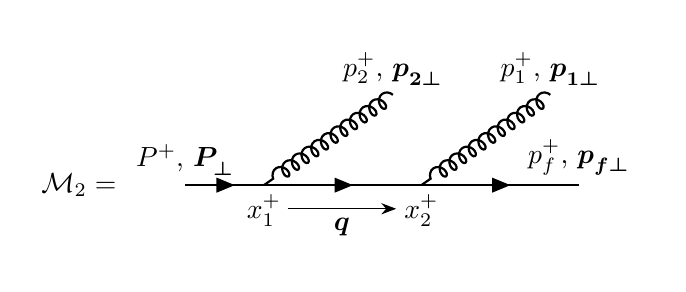
\begin{tikzpicture}\begin{feynman}
		
		% ---------------------
		% Proper size --- Bounding box
		\useasboundingbox (-2.0cm, -1.0cm) rectangle (6.0cm, 2.0cm);	
		
		% ---------------------
		% Blob & Shower origin
		
		\coordinate (Start) at (0.00cm,0.00cm);
		
		\path (Start) +(1.00cm,0.00cm) coordinate (Split1);
		\path (Split1) +(2.00cm,0.00cm) coordinate (Split2);
		\path (Split2) +(2.00cm,0.00cm) coordinate (Quarkf);
		
		\path (Split1) +(35:2.00cm) coordinate (Gluon1);
		\path (Split2) +(35:2.00cm) coordinate (Gluon2);
		
		\vertex[left=0.75cm of Start] (M2) {$\mathcal{M}_2 = $};
		
		\vertex[above=0cm of Start] (Qi) {$ P^{+}_{}\text{, } \boldsymbol{ P_{\perp}^{}} $};
		\vertex[above=0cm of Gluon1] (G1) {$ p^{+}_{2}\text{, } \boldsymbol{ p_{2\perp}^{}} $};
		\vertex[above=0cm of Gluon2] (G2) {$ p^{+}_{1}\text{, } \boldsymbol{ p_{1\perp}^{}} $};
		\vertex[above=0cm of Quarkf] (Qf) {$ p^{+}_{f}\text{, } \boldsymbol{ p_{f\perp}^{}} $};
		
		\vertex[below=0.0cm of Split1] (S1) {$x^+_1$};
		\vertex[below=0.0cm of Split2] (S2) {$x^+_2$};
		% ---------------------	
		\diagram*{
			
			(Start) -- [thick, fermion] (Split1)
			-- [thick, fermion, momentum'=$ \boldsymbol{ q_{}^{}} $] (Split2)
			-- [thick, fermion] (Quarkf),
			
			(Gluon1) -- [thick, gluon] (Split1),
			(Gluon2) -- [thick, gluon] (Split2),
			
		};
		
		
		
\end{feynman}\end{tikzpicture}

% Set this figure's name when externalised 
\tikzsetnextfilename{double-emission-M3} 


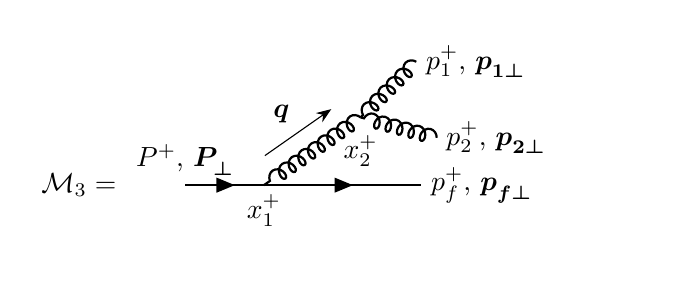
\begin{tikzpicture}\begin{feynman}
		
		% ---------------------
		% Proper size --- Bounding box
		\useasboundingbox (-2.0cm, -1.0cm) rectangle (6.0cm, 2.0cm);	
		
		% ---------------------
		% Blob & Shower origin
		
		\coordinate (Start) at (0.00cm,0.00cm);
		
		\path (Start) +(1.00cm,0.00cm) coordinate (Split1);
		\path (Split1) +(2.00cm,0.00cm) coordinate (Quarkf);
		\path (Split1) +(35:1.50cm) coordinate (Split2);
		
		\path (Split2) +(+45:1.00cm) coordinate (Gluon1);
		\path (Split2) +(-15:1.00cm) coordinate (Gluon2);

		\vertex[left=0.75cm of Start] (M3) {$\mathcal{M}_3 = $};
		
		\vertex[above=0cm of Start] (Qi) {$ P^{+}_{}\text{, } \boldsymbol{ P_{\perp}^{}} $};
		\vertex[right=0cm of Gluon1] (G1) {$ p^{+}_{1}\text{, } \boldsymbol{ p_{1\perp}^{}} $};
		\vertex[right=0cm of Gluon2] (G2) {$ p^{+}_{2}\text{, } \boldsymbol{ p_{2\perp}^{}} $};
		\vertex[right=0cm of Quarkf] (Qf) {$ p^{+}_{f}\text{, } \boldsymbol{ p_{f\perp}^{}} $};
		
		\vertex[below=0.00cm of Split1] (S1) {$x^+_1$};
		\vertex[below=0.10cm of Split2] (S2) {$x^+_2$};
		
		% ---------------------	
		\diagram*{
			
			(Start) -- [thick, fermion] (Split1)
					-- [thick, fermion] (Quarkf),
			
			(Split2) -- [thick, gluon, rmomentum'=$\boldsymbol{q}$] (Split1),
			
			(Gluon1) -- [thick, gluon] (Split2),
			(Gluon2) -- [thick, gluon] (Split2),
			
		};
		
		
		
\end{feynman}\end{tikzpicture}

\end{document}
